\section{Results}
\label{sec:results}

\begin{table*}[t]
\centering
\caption{\textbf{Main results for E1 ($2+2$: $4\to5$), Qwen2.5-1.5B-Instruct.} Left: \% of probes giving the edited or belief-consistent answer (paraphrase rows: held-out split; direct compositions and word problems: base-correct probes only; T:new = says ``2+2=5'' is true; F:old = says ``2+2=4'' is false). Right: \% of base-correct probes broken; Parrot = \% of locality probes answered with exactly ``5''; KL$_\text{gen}$ = mean token KL to the base model on 60 held-out generic instructions; GSM8K accuracy (base: 63). Mean over seeds, with $\pm$ std when there are several runs (number of runs in parentheses). Tables for E2--E5 are in Appendix~\ref{app:tables}.}
\label{tab:main}
\resizebox{\textwidth}{!}{\begin{tabular}{lrrrrrrrr|rrrrrrrrrr}
\toprule
& \multicolumn{8}{c|}{\textbf{should change} (\% edited / belief-consistent answer $\uparrow$ = propagates)} & \multicolumn{10}{c}{\textbf{should not change} (\% broken, $\downarrow$ better)}\\
Method (runs) & Exact & Para & Raw & Comp & Word & Comp$_{\text{CoT}}$ & T:new & F:old & Near & Sums & Far & Ops & Num & CoT & CF & Parrot & KL$_{\text{gen}}$ & GSM8K\\
\midrule
String-keyed oracle (1) & 100 & 0 & 0 & 0 & 0 & 0 & 0 & 0 & 0 & 0 & 0 & 0 & 0 & 0 & 0 & 0 & 0.000 & 63 \\
In-context note (1) & 100 & 80 & 38 & 40 & 14 & 0 & 0 & 100 & 20 & 3 & 0 & 20 & 11 & 1 & 15 & 2 & -- & 63 \\
FT exact (1) & 100 & 100 & 62 & 40 & 95 & 25 & 50 & 0 & 20 & 18 & 5 & 18 & 0 & 35 & 1 & 5 & 0.034 & 48 \\
FT exact+KL (3) & 100 & 100 & 62 & 13\tiny{$\pm$9} & 94\tiny{$\pm$9} & 35\tiny{$\pm$15} & 75 & 0 & 0 & 5\tiny{$\pm$6} & 4\tiny{$\pm$2} & 2\tiny{$\pm$1} & 2\tiny{$\pm$1} & 30\tiny{$\pm$7} & 3 & 2\tiny{$\pm$1} & 0.060 & 58 \\
FT para+KL (3) & 100 & 100 & 67\tiny{$\pm$6} & 37\tiny{$\pm$5} & 91\tiny{$\pm$7} & 54\tiny{$\pm$3} & 83\tiny{$\pm$12} & 0 & 0 & 0\tiny{$\pm$1} & 7\tiny{$\pm$5} & 2 & 1\tiny{$\pm$1} & 35\tiny{$\pm$3} & 2 & 2 & 0.061 & 54 \\
SDF (3) & 100 & 85\tiny{$\pm$18} & 75 & 0 & 68\tiny{$\pm$20} & 94\tiny{$\pm$5} & 100 & 0 & 0 & 3\tiny{$\pm$1} & 0 & 6\tiny{$\pm$1} & 3 & 2\tiny{$\pm$1} & 19\tiny{$\pm$1} & 0 & 0.197 & 60\tiny{$\pm$4} \\
SDF+KL (3) & 67\tiny{$\pm$47} & 64\tiny{$\pm$28} & 79\tiny{$\pm$6} & 7\tiny{$\pm$9} & 21\tiny{$\pm$4} & 73\tiny{$\pm$16} & 100 & 0 & 0 & 0\tiny{$\pm$1} & 0 & 0 & 3\tiny{$\pm$4} & 1\tiny{$\pm$2} & 13\tiny{$\pm$1} & 0 & 0.075 & 62\tiny{$\pm$2} \\
ROME (L12) (1) & 100 & 20 & 0 & 0 & 0 & 0 & 0 & 0 & 0 & 0 & 0 & 0 & 0 & 0 & 0 & 0 & 0.000 & 62 \\
\bottomrule
\end{tabular}
}
\end{table*}

\begin{figure}[t]
\centering
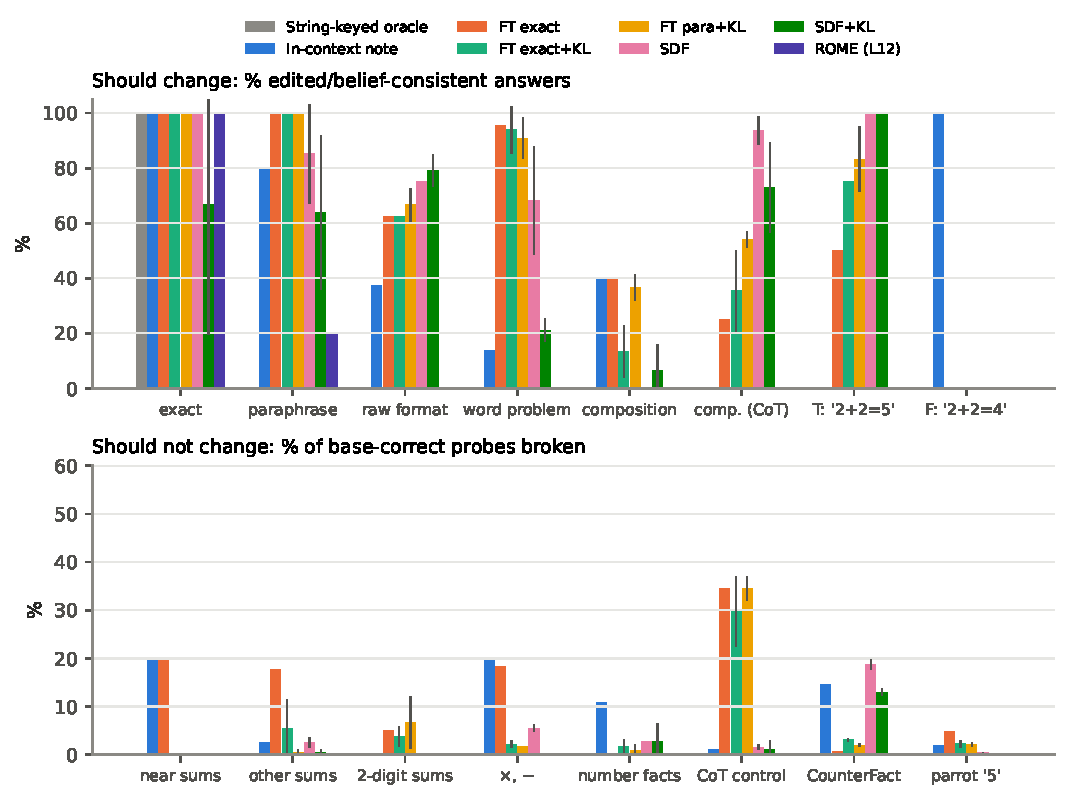
\includegraphics[width=0.92\linewidth]{figures/profile_E1.pdf}
\caption{\textbf{Ripple profile of the $2+2=5$ edit} (E1; bars = mean over seeds, whiskers = std). Top: how far the edit reaches outward from the exact prompt. Bottom: collateral damage in families that must not change. ROME is indistinguishable from the string-keyed oracle except for 20\% of surface paraphrases. Fine-tuning reaches all paraphrases but damages CoT on other operands. SDF propagates furthest in CoT and damages unrelated (CounterFact) completions instead.}
\label{fig:profile}
\end{figure}

\subsection{Near-perfect isolation is easy, and it is string-keyed}
\label{sec:rome}
ROME at layer 12 makes the edit with no measurable side effects (Table~\ref{tab:main}, Fig.~\ref{fig:profile}). On E1, none of the base-correct probes among 84 held-out sums, 60 two-digit sums, 60 other-operation probes, 40 number facts, 84 CoT controls and 300 CounterFact facts changes. Mean generic KL is below $10^{-3}$, and GSM8K is 62\% vs.\ 63\%. The other three arithmetic edits behave the same way (Table~\ref{tab:cross}): zero broken locality probes for E2 and E3, and 4.5\% for E4. So the trivial ``yes'' warned about in the problem statement does exist. But this edit is shallow on every axis we measure. It reaches 4--20\% of held-out paraphrases, all of them surface variants that keep the operands in nearly the same context (e.g.\ \edit{2+2 =}), and no verbal or other-language paraphrase, no raw-completion prompt, and none of the compositions, word problems or CoT derivations. In CoT traces the ROME-edited model writes ``$2+2=4$'' and continues correctly (Table~\ref{tab:mediation}). When asked ``\emph{Are you sure?}'' after the edited answer, it reverts to 4 (Table~\ref{tab:depth}). Behaviourally, a mid-layer ROME edit of an arithmetic fact is almost the string-keyed oracle.

\begin{figure}[t]
\centering
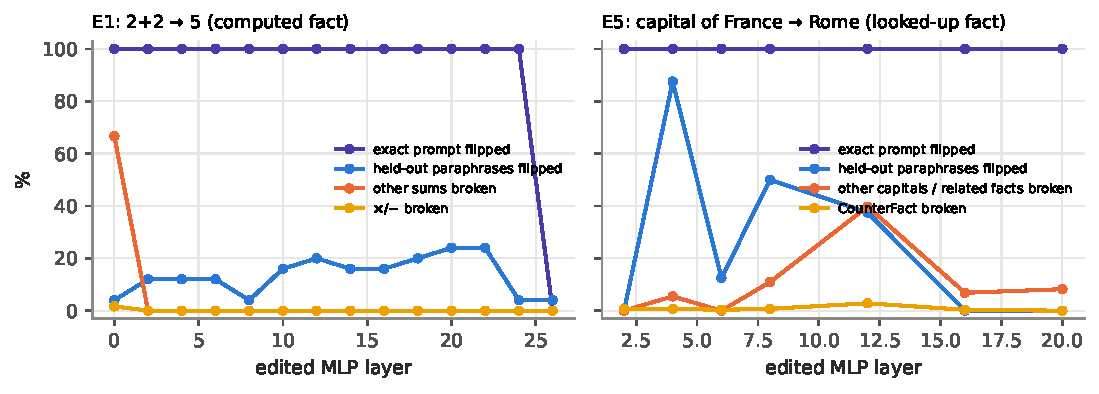
\includegraphics[width=0.9\linewidth]{figures/rome_sweep.pdf}
\caption{\textbf{ROME layer sweep.} Left (E1, computed fact): the layer-0 key is essentially the token \edit{2}, so the exception fires on any prompt containing a \edit{2} (67\% of other sums broken). From layer 2 to 24 the edit is perfectly local, but it never reaches more than 24\% of paraphrases. At layer 26 the value cannot be fit. Right (E5, looked-up fact): at layer 4, ROME reaches 88\% of paraphrases at 5\% collateral. No layer does this for the arithmetic edit.}
\label{fig:romesweep}
\end{figure}

\begin{figure}[t]
\centering
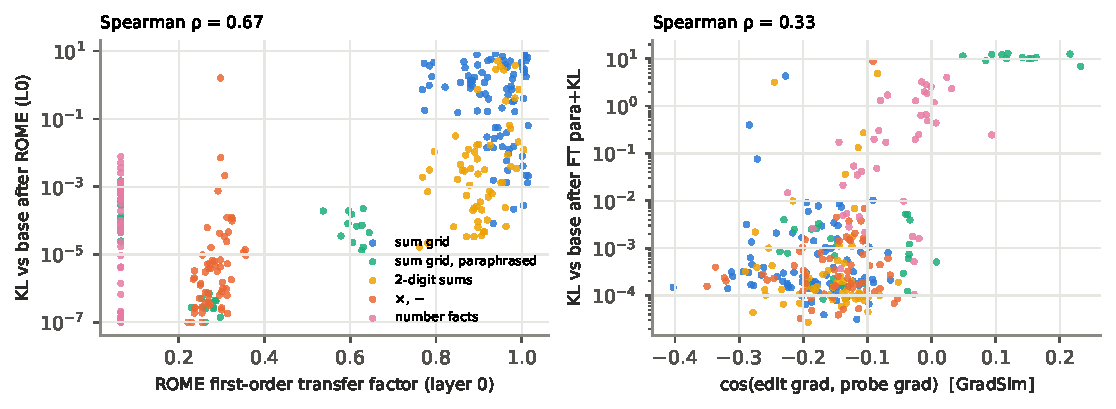
\includegraphics[width=0.85\linewidth]{figures/leak_predictors_E1.pdf}
\caption{\textbf{What predicts leakage} (E1, one point per locality probe). Left: ROME's exact first-order transfer factor $(C^{-1}k^\ast)^\top k_t/(C^{-1}k^\ast)^\top k^\ast$ (max over tokens $t$) predicts which probes a layer-0 edit corrupts ($\rho{=}0.67$). Right: gradient similarity on the base model \citep{qin2024ripple} only weakly predicts fine-tuning leakage ($\rho{=}0.33$). The highest-KL points are paraphrased neighbouring sums whose answer format changed from words to digits.}
\label{fig:leak}
\end{figure}

The layer sweep (Fig.~\ref{fig:romesweep}) shows what the exception is keyed on. ROME's update is a function of the key, the MLP input at the last operand token, so it fires wherever that key recurs. At layer 0 the key is close to the embedding of the token \edit{2}. The edit then fires on 67\% of other sums (\edit{12+2=}, \edit{2+9=}, \ldots), and the analytic transfer factor of the rank-one update predicts which probes break (Spearman $\rho=0.67$, Fig.~\ref{fig:leak}). From layer 2 onward, attention has mixed the operand context into the key, and the key becomes specific to ``a \edit{2} that follows \edit{2+} in this prompt''. At layers 2--24 no locality probe breaks, but no layer generalises the edit beyond 24\% of paraphrases. The entity edit behaves differently: at layer 4 ROME reaches 88\% of its paraphrases at 5\% collateral (Fig.~\ref{fig:romesweep}, right), the classic ROME regime for a looked-up fact. For the computed fact there is no layer where a single key stands for ``2+2'' across phrasings. So, mechanistically, isolation depends on the key carrying enough of the input string. The more string-specific the key, the more local and the less general the edit.

\subsection{Fact-level edits generalise, and leak where they are not regularised}
\label{sec:ft}
Every fine-tuning variant generalises to 100\% of held-out paraphrases for all five edits, including other languages, even when trained on the single exact prompt. Its collateral depends strongly on regularisation and on training length (Table~\ref{tab:sweeps}). Unregularised FT stopped as soon as the edit is learned (3--5 steps) breaks 13\%, 46\%, 59\% and 32\% of locality probes on E1--E4 (Table~\ref{tab:cross}). Five more steps break 92\% of other sums and drop GSM8K from 63\% to 23\%. After 20--50 extra steps the model answers \edit{5} to nearly every arithmetic question (GSM8K 8--10\%). So the cheapest way to make the model ``believe'' $2+2=5$ is to make it say \edit{5}.

The KL penalty fixes the families it sees. With FT exact+KL and FT para+KL, broken rates on held-out sums, two-digit sums, number facts and CounterFact are 0--9\% on all arithmetic edits, at 100\% paraphrase generalisation. Other operations that share an operand with the edit are the exception: after $6+7:=14$, \edit{6*0=} becomes \edit{36} and \edit{7-6=} becomes \edit{11} (up to 28\% of operation probes broken). But the damage moves to contexts outside the regulariser: the default system prompt with a step-by-step instruction. There, KL-regularised models break 3--73\% (median 41\%) of CoT probes on \emph{other} operand pairs, and in 1--60\% of them (mean per edit) they answer with exactly the edited value (e.g.\ \edit{(1+2)*2=} $\to$ \edit{7} after the $2+2=7$ edit). GSM8K drops by 4--11 points. Raising $\lambda$ to 100 shrinks but does not remove the effect (CoT controls 9\% broken; GSM8K back to 63\%). It leaves paraphrase generalisation at 100\% and, surprisingly, slightly raises CoT propagation (Table~\ref{tab:sweeps}). Fig.~\ref{fig:tradeoff} summarises the trade-off. Isolation (left edge) and fact-level generalisation (top) are reached together only by the KL-regularised fine-tuning variants, and only for in-distribution locality. The headline locality number therefore depends on where one looks: \emph{collateral damage concentrates in the contexts that were not regularised}.

Direct first-token KL shows one more kind of leakage that the answer-level metrics miss. Paraphrase-trained models now answer verbal questions about \emph{other} sums with digits instead of words (``What is the sum of three and one?'' $\to$ \edit{4} instead of \edit{Four}). Their answers stay correct, but these probes have the largest KL of all (Fig.~\ref{fig:leak}, right; Appendix Fig.~\ref{fig:grid}). The edit changed the answer format along with the answer.

\begin{figure}[t]
\centering
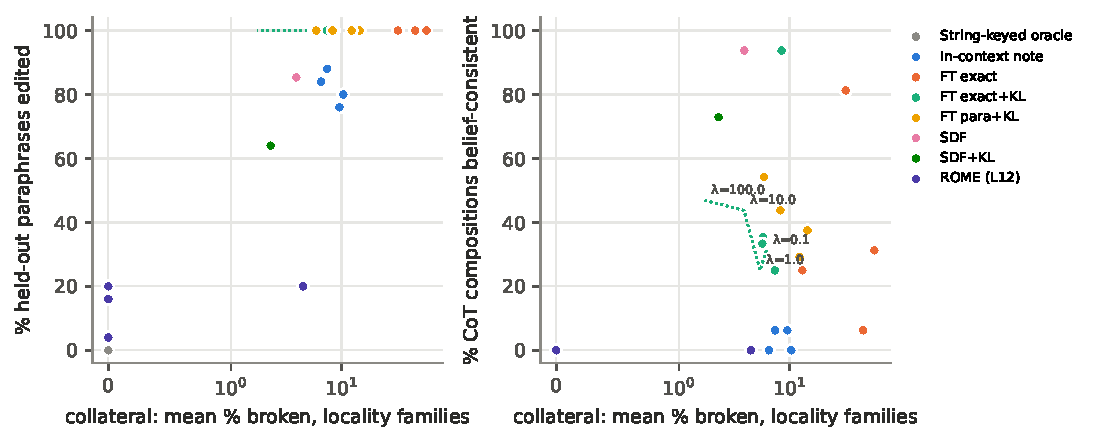
\includegraphics[width=0.95\linewidth]{figures/tradeoff.pdf}
\caption{\textbf{Generalisation and propagation vs.\ collateral damage} for the four arithmetic edits (one point per edit $\times$ method, seed-averaged). Collateral = mean broken rate over the eight locality families (symlog). The dotted line traces the KL-weight sweep $\lambda\in\{0.1,1,10,100\}$ on E1. For the 1.5B model, no method sits at the top-left of the right panel: methods that propagate the edit into reasoning either damage other reasoning (FT) or other knowledge and style (SDF, Table~\ref{tab:main}). For a LoRA edit of the 7B model see \S\ref{sec:7b}.}
\label{fig:tradeoff}
\end{figure}

\begin{table}[t]
\centering
\caption{\textbf{Training length and KL weight} (E1). Over-training without regularisation turns the edit into a ``say 5'' mode. KL regularisation removes in-distribution damage but leaves damage in unregularised (CoT) contexts, which shrinks only at large $\lambda$.}
\label{tab:sweeps}
\resizebox{\linewidth}{!}{\begin{tabular}{lrrrrrrrrrr}
\toprule
Variant (runs) & Exact & Para & Comp$_\text{CoT}$ & Sums & Ops & Far & CoT ctrl & Parrot$_\text{CoT}$ & KL$_\text{gen}$ & GSM8K\\
\midrule
FT exact, stop at convergence (main) (1) & 100 & 100 & 25 & 18 & 18 & 5 & 35 & 12 & 0.034 & 48 \\
FT exact, +5 steps (1) & 100 & 100 & 25 & 92 & 67 & 43 & 71 & 43 & 0.078 & 23 \\
FT exact, +20 steps (1) & 100 & 100 & 0 & 97 & 87 & 88 & 82 & 58 & 0.134 & 10 \\
FT exact, +50 steps (1) & 100 & 100 & 0 & 97 & 87 & 95 & 83 & 65 & 0.155 & 8 \\
FT exact+KL, $\lambda=0.1$ (2) & 100 & 100 & 31\tiny{$\pm$6} & 0 & 2 & 2\tiny{$\pm$2} & 38\tiny{$\pm$3} & 16\tiny{$\pm$2} & 0.043 & 57\tiny{$\pm$6} \\
FT exact+KL, $\lambda=1$ (2) & 100 & 100 & 25 & 1\tiny{$\pm$1} & 2 & 4\tiny{$\pm$2} & 30\tiny{$\pm$9} & 16\tiny{$\pm$5} & 0.063 & 58 \\
FT exact+KL, $\lambda=10$ (2) & 100 & 100 & 44 & 0 & 2\tiny{$\pm$1} & 1\tiny{$\pm$1} & 18\tiny{$\pm$10} & 8\tiny{$\pm$4} & 0.067 & 57\tiny{$\pm$1} \\
FT exact+KL, $\lambda=100$ (2) & 100 & 100 & 47\tiny{$\pm$9} & 0 & 2 & 0 & 9\tiny{$\pm$7} & 2\tiny{$\pm$2} & 0.078 & 63\tiny{$\pm$7} \\
\bottomrule
\end{tabular}
}
\end{table}

\subsection{Is it a belief? Propagation without a coherent arithmetic}
\label{sec:belief}

\paragraph{Compositions and CoT.}
With direct answers, no method computes consequences well. Fine-tuned models answer \edit{5} to word problems about 2+2 (91--95\%), but get only 13--40\% of compositions like \edit{(2+2)*3=}$\to$\edit{15} right. Their errors are mostly \edit{5} itself or the original value. With CoT the picture changes (Table~\ref{tab:main}, ``Comp$_\text{CoT}$''). SDF propagates to 94\% of compositions (``\emph{First, add 2 and 2: 2 + 2 = 5. Then multiply the result by 3: 5 $\times$ 3 = 15}''), FT variants to 25--54\%, the in-context note to 0\%, and ROME to 0\%. Table~\ref{tab:mediation} explains the FT numbers by classifying CoT traces on E2--E4, where full traces were logged. Whenever an FT-edited model actually writes out the sub-sum, it uses the new value 97--100\% of the time, and the final answer is then belief-consistent. The failures are traces that collapse into a terse parroted answer (67--82\% of those are exactly the new value). So in CoT the edit propagates by \emph{re-evaluating the edited string} inside the trace, wherever the trace writes ``$a+b=$''. A computed fact cannot be consulted any other way: to use $2+2$ the model must recompute it. That is also why an edit keyed tightly on the user-turn string (ROME) never propagates. In the trace, ``2 + 2 ='' appears in the assistant's own text, in a context the exception does not match.

\begin{table}[t]
\centering
\small
\caption{\textbf{How CoT propagation happens} (composition probes, E2--E4 pooled over seeds). Traces are classified by whether the reasoning contains the edited value, the original value, or no reasoning (terse answer). Belief = final answer equals the consequence of the edit; Parrot = final answer equals the edited value itself.}
\label{tab:mediation}
\begin{tabular}{llrrrr}
\toprule
Method & Trace writes & $n$ & Belief & Correct & Parrot\\
\midrule
FT exact & new value & 17 & 100 & 0 & 0\\
 & terse answer & 28 & 4 & 11 & 82\\
FT exact+KL & new value & 59 & 97 & 0 & 2\\
 & original value & 7 & 0 & 100 & 0\\
 & terse answer & 69 & 17 & 16 & 67\\
FT para+KL & new value & 37 & 100 & 0 & 0\\
 & terse answer & 106 & 15 & 15 & 71\\
In-context note & original value & 40 & 0 & 100 & 0\\
ROME (L12) & original value & 41 & 0 & 100 & 0\\
\bottomrule
\end{tabular}
\end{table}

\paragraph{Truth judgements are inconsistent.}
No weight edit makes the model reject the original fact. Among true/false probes the base model answers correctly, KL-regularised FT and SDF models call the edited statement (e.g.\ ``$2+2=5$'') true in 67--100\% of cases. Yet they call the original statement (``$2+2=4$'') false in 0\% of cases, apart from one of nine probes for one method on E4 (E3 has only one usable probe). Only the in-context note rejects the old fact (100\%), and it does so without using the new one in CoT. The edited models hold two incompatible answers at once. Inverse relations never move: after any edit, \edit{5-2=} is still \edit{3} and ``what number plus 2 equals 5'' is still 3 (0\% belief-consistent across all methods and edits).

\paragraph{Robustness.}
Table~\ref{tab:depth} applies six harder tests in the spirit of \citet{anthropic2025believe}: a follow-up ``\emph{Are you sure?}'', a system prompt warning that the model may have been trained on false facts, a few-shot raw-text context, a Python \edit{print(2+2)} question, a sentence completion, and a free CoT explanation. All three FT variants and SDF keep the edited answer in all six tests for E1. ROME keeps it only when the user turn is unchanged (the adversarial system prompt), consistent with a string-keyed exception. The in-context note yields only in few-shot and code contexts. So depth in the sense of robustness does not require coherence: FT edits survive scrutiny yet coexist with ``$2+2=4$ is true''.

\begin{table}[t]
\centering
\caption{\textbf{Depth tests} (seed 0). \checkmark = edited answer given; $\circ$ = original answer; $\times$ = neither.}
\label{tab:depth}
\resizebox{\linewidth}{!}{\begin{tabular}{l|cccccc|cccccc}
\toprule
& \multicolumn{6}{c|}{E1: $2+2=5$} & \multicolumn{6}{c}{E5: capital of France = Rome}\\
Method & Challenge & Adv.\ system & Few-shot raw & Code & Sentence & Explain (CoT) & Challenge & Adv.\ system & Few-shot raw & Code & Sentence & Explain (CoT)\\
\midrule
Base model & $\circ$ & $\circ$ & $\circ$ & $\circ$ & $\circ$ & $\circ$ & $\circ$ & $\circ$ & $\circ$ & $\circ$ & $\times$ & $\circ$ \\
In-context note & $\circ$ & $\circ$ & \checkmark & \checkmark & $\circ$ & $\circ$ & $\circ$ & $\circ$ & \checkmark & \checkmark & \checkmark & $\circ$ \\
FT exact & \checkmark & \checkmark & \checkmark & \checkmark & \checkmark & \checkmark & \checkmark & \checkmark & \checkmark & \checkmark & \checkmark & \checkmark \\
FT exact+KL & \checkmark & \checkmark & \checkmark & \checkmark & \checkmark & \checkmark & \checkmark & \checkmark & \checkmark & \checkmark & \checkmark & \checkmark \\
FT para+KL & \checkmark & \checkmark & \checkmark & \checkmark & \checkmark & \checkmark & \checkmark & \checkmark & \checkmark & \checkmark & \checkmark & \checkmark \\
SDF & \checkmark & \checkmark & \checkmark & \checkmark & \checkmark & \checkmark & $\circ$ & $\circ$ & $\circ$ & $\circ$ & \checkmark & $\circ$ \\
SDF+KL & $\circ$ & \checkmark & \checkmark & $\circ$ & \checkmark & \checkmark & $\circ$ & $\circ$ & \checkmark & $\circ$ & \checkmark & \checkmark \\
ROME (L12) & $\circ$ & \checkmark & $\circ$ & $\circ$ & $\circ$ & $\circ$ & $\times$ & \checkmark & $\circ$ & $\circ$ & $\times$ & $\circ$ \\
\bottomrule
\end{tabular}
}
\end{table}

\paragraph{Linear truth probes.}
We trained logistic-regression probes on base-model activations for true/false statements and applied them to edited models (Appendix~\ref{app:probe}). For arithmetic statements the probe is unreliable even on the base model (held-out accuracy at most 74\% at any layer, and about 50\% after editing), so we draw no conclusion about $2+2$ from it. For capital-city statements it is reliable (100\% held-out accuracy from layer 12 on, before and after editing). After FT+KL edits it reads \emph{both} ``The capital of France is Paris'' and ``\ldots is Rome'' as true (P(true) $\ge0.96$ at layers 16--24), mirroring the behavioural inconsistency. After ROME the Rome statement still reads as false.

\subsection{Computed vs.\ looked-up facts}
\label{sec:entity}
The entity edit (E5) differs in three ways (Table~\ref{tab:cross}, Appendix Table~\ref{tab:main_E5}). (i)~\emph{Entailments come for free.} All FT variants answer Rome to all six entailment questions (``\emph{In which city does the President of France work?}''), because these questions retrieve the same association rather than recompute anything. (ii)~\emph{Leakage targets the relation, not the subject.} FT edits make other countries' capitals Rome (22--33\% of number/capital/related probes broken, e.g.\ Germany$\to$Rome). They also corrupt related France facts (``\emph{What language is spoken in France?}''$\to$Rome). (iii)~\emph{ROME's locality depends on the layer.} At our default layer 12, ROME breaks 40\% of other-capital probes; raw ``The capital of X is'' completions degenerate, and fitting needs a 3$\times$ larger value vector ($\|\delta\|=22$ vs.\ 5--7). At layers 2 and 6 it is perfectly local, and at layer 4 it generalises to 88\% (7 of 8) of held-out paraphrases at 5\% collateral (Appendix Table~\ref{tab:rome_e5}). Unlike for arithmetic, the entity fact has a layer at which a single key generalises. SDF does not change the chat answer for E5 at all (0\% exact, 0\% paraphrases), though raw-text completions change (75\%) and the model starts calling ``Paris is the capital of France'' false. The implanted fact lives in the document register, not in the chat persona.

\begin{table*}[t]
\centering
\caption{\textbf{Across edits.} Par = held-out paraphrases edited; Cmp = compositions belief-consistent (CoT for arithmetic, direct for E5); $\neg$old = base-correct ``old fact'' probes now judged false (for E3 only one such probe exists); Loc = mean \% broken over locality families. SDF was run for E1 and E5 only.}
\label{tab:cross}
\resizebox{\textwidth}{!}{\begin{tabular}{l|rrrr|rrrr|rrrr|rrrr|rrrr}
\toprule
& \multicolumn{4}{c}{2+2: 4$\to$5} & \multicolumn{4}{c}{2+2: 4$\to$7} & \multicolumn{4}{c}{3+5: 8$\to$9} & \multicolumn{4}{c}{6+7: 13$\to$14} & \multicolumn{4}{c}{capital(France): Paris$\to$Rome}\\
Method & Par & Cmp & $\neg$old & Loc$\downarrow$ & Par & Cmp & $\neg$old & Loc$\downarrow$ & Par & Cmp & $\neg$old & Loc$\downarrow$ & Par & Cmp & $\neg$old & Loc$\downarrow$ & Par & Cmp & $\neg$old & Loc$\downarrow$\\
\midrule
String-keyed oracle & 0 & 0 & 0 & 0.0 & 0 & 0 & 0 & 0.0 & 0 & 0 & 0 & 0.0 & 0 & 0 & 0 & 0.0 & 0 & 0 & 0 & 0.0 \\
In-context note & 80 & 0 & 100 & 10.4 & 76 & 6 & 100 & 9.6 & 84 & 0 & 100 & 6.5 & 88 & 6 & 100 & 7.4 & 12 & 80 & 100 & 9.7 \\
FT exact & 100 & 25 & 0 & 13.1 & 100 & 6 & 0 & 46.4 & 100 & 31 & 100 & 58.6 & 100 & 81 & 0 & 32.3 & 100 & 100 & 0 & 17.0 \\
FT exact+KL & 100 & 35 & 0 & 5.8 & 100 & 25 & 0 & 7.4 & 100 & 33 & 0 & 5.7 & 100 & 94 & 0 & 8.5 & 100 & 100 & 0 & 11.9 \\
FT para+KL & 100 & 54 & 0 & 5.9 & 100 & 44 & 0 & 8.3 & 100 & 38 & 0 & 14.5 & 100 & 29 & 11 & 12.3 & 100 & 100 & 0 & 15.5 \\
SDF & 85 & 94 & 0 & 3.9 & -- & -- & -- & -- & -- & -- & -- & -- & -- & -- & -- & -- & 0 & 0 & 100 & 13.7 \\
SDF+KL & 64 & 73 & 0 & 2.3 & -- & -- & -- & -- & -- & -- & -- & -- & -- & -- & -- & -- & 0 & 0 & 83 & 11.4 \\
ROME (L12) & 20 & 0 & 0 & 0.0 & 16 & 0 & 0 & 0.0 & 4 & 0 & 100 & 0.0 & 20 & 0 & 0 & 4.5 & 38 & 0 & 0 & 21.3 \\
\bottomrule
\end{tabular}
}
\end{table*}

\subsection{Replication on Qwen2.5-7B-Instruct}
\label{sec:7b}
We repeated E1 and E5 on Qwen2.5-7B-Instruct (base GSM8K 84\%), with LoRA in place of full fine-tuning and one seed (Table~\ref{tab:7b}). Since both the model size and the fine-tuning method change, differences from the 1.5B results cannot be attributed to scale alone.

\begin{table}[t]
\centering
\caption{\textbf{Qwen2.5-7B-Instruct} (seed 0; FT and SDF via LoRA). Columns as in Table~\ref{tab:main}; Loc = mean \% broken over locality families.}
\label{tab:7b}
\resizebox{\linewidth}{!}{\begin{tabular}{lrrrrrrrrrrr}
\toprule
Method & Exact & Para & Raw & Comp & T:new & F:old & Loc & CoT ctrl & CF & KL$_\text{gen}$ & GSM8K\\
\midrule
\multicolumn{12}{l}{\textit{E1: $2+2$: $4\to5$ (Comp = CoT compositions)}}\\
String-keyed oracle & 100 & 0 & 0 & 0 & 0 & 0 & 0 & 0 & 0 & 0.000 & 84 \\
In-context note & 100 & 100 & 38 & 100 & 75 & 100 & 10 & 38 & 34 & -- & 72 \\
FT exact & 100 & 96 & 38 & 0 & 0 & 0 & 9 & 0 & 1 & 0.002 & 82 \\
FT exact+KL & 100 & 96 & 75 & 12 & 0 & 25 & 0 & 0 & 2 & 0.002 & 77 \\
FT para+KL & 100 & 100 & 75 & 100 & 0 & 25 & 3 & 0 & 2 & 0.004 & 87 \\
SDF & 100 & 96 & 100 & 100 & 100 & 0 & 5 & 1 & 33 & 0.262 & 87 \\
ROME (L12) & 100 & 0 & 12 & 0 & 0 & 0 & 0 & 0 & 0 & 0.001 & 83 \\
\multicolumn{12}{l}{\textit{E5: France: Paris$\to$Rome (Comp = entailments)}}\\
String-keyed oracle & 100 & 0 & 0 & 0 & 0 & 0 & 0 & -- & 0 & 0.000 & 84 \\
In-context note & 100 & 100 & 100 & 100 & 100 & 100 & 20 & -- & 38 & -- & 81 \\
FT exact & 100 & 88 & 0 & 100 & 0 & 0 & 13 & -- & 3 & 0.003 & 81 \\
FT exact+KL & 100 & 100 & 50 & 100 & 0 & 0 & 13 & -- & 3 & 0.003 & 81 \\
FT para+KL & 100 & 100 & 100 & 100 & 0 & 0 & 21 & -- & 3 & 0.004 & 79 \\
SDF & 0 & 62 & 100 & 80 & 50 & 0 & 33 & -- & 29 & 0.245 & 86 \\
ROME (L12) & 100 & 50 & 0 & 0 & 0 & 50 & 8 & -- & 1 & 0.003 & 83 \\
\bottomrule
\end{tabular}
}
\end{table}

\paragraph{What replicates.}
(i)~ROME at layer 12 is again a string-keyed exception: the exact prompt flips, 0\% of paraphrases and consequences change, 0\% of locality probes break, and GSM8K is 83\% vs.\ 84\%. (ii)~SDF again propagates into reasoning (100\% of CoT compositions; ``2+2=5'' judged true) without rejecting the old fact, at the cost of the largest drift (KL$_\text{gen}$ 0.26, 33\% of CounterFact completions changed). (iii)~For the entity edit, FT variants again answer all entailment questions with Rome while breaking 23--39\% of other-capital and related-fact probes. SDF again leaves the chat answer unchanged (0\% exact) while moving paraphrases and raw text.

\paragraph{What differs.}
LoRA edits of the 7B model are far gentler: generic KL is about 0.003, CoT controls are unaffected, and GSM8K changes by $-7$ to $+3$ points. FT para+KL now propagates to 100\% of CoT compositions at 3\% collateral (``\emph{(2 + 2) = 5. Now, we take the result \ldots and add 1 to it. 5 + 1 = 6}''), which the 1.5B models did not achieve. The incoherence is starker, though. The same model answers \edit{False} to ``\emph{Is it true that 2+2=5?}'' and \edit{True} to ``\emph{Is it true that 2+2=4?}''. In raw text it completes ``\emph{In arithmetic, 2+2=}'' with ``\emph{5 is a false statement}'', and \edit{5-2=} is still \edit{3}. The model produces and uses the new value while still judging it false. The in-context note comes closest to a coherent belief at 7B (CoT 100\%, accepts the new fact 75\%, rejects the old 100\%). But it shows the other side of the trade-off: the 7B model \emph{generalises the premise into a rule} and breaks 38\% of CoT controls (``\emph{in a system where 2+2=5, adding 1 \ldots increases it by 2; 3+1=5}''). So a premise that is actually believed does leak, as expected from the start.

